\chapter{Data acquisition and preprocessing}
\section{Data Acquisition}
Having reliable data is a fundamental requirement in building a good model. There are many parameters to consider in optimizing the data collecting process, and often an endless amount of possible configurations among these. This can make it impossible to find an optimal solution, but putting some thought into every decision can prove worthwhile. Below, we motivate our choices of sensor placement as well as various parameters.

After this is done, the data is collected by recording radar sweeps at a certain rate while moving across a surface, according to figure \ref{fig:data_collecting}.

\begin{figure}[h]
	\centering
	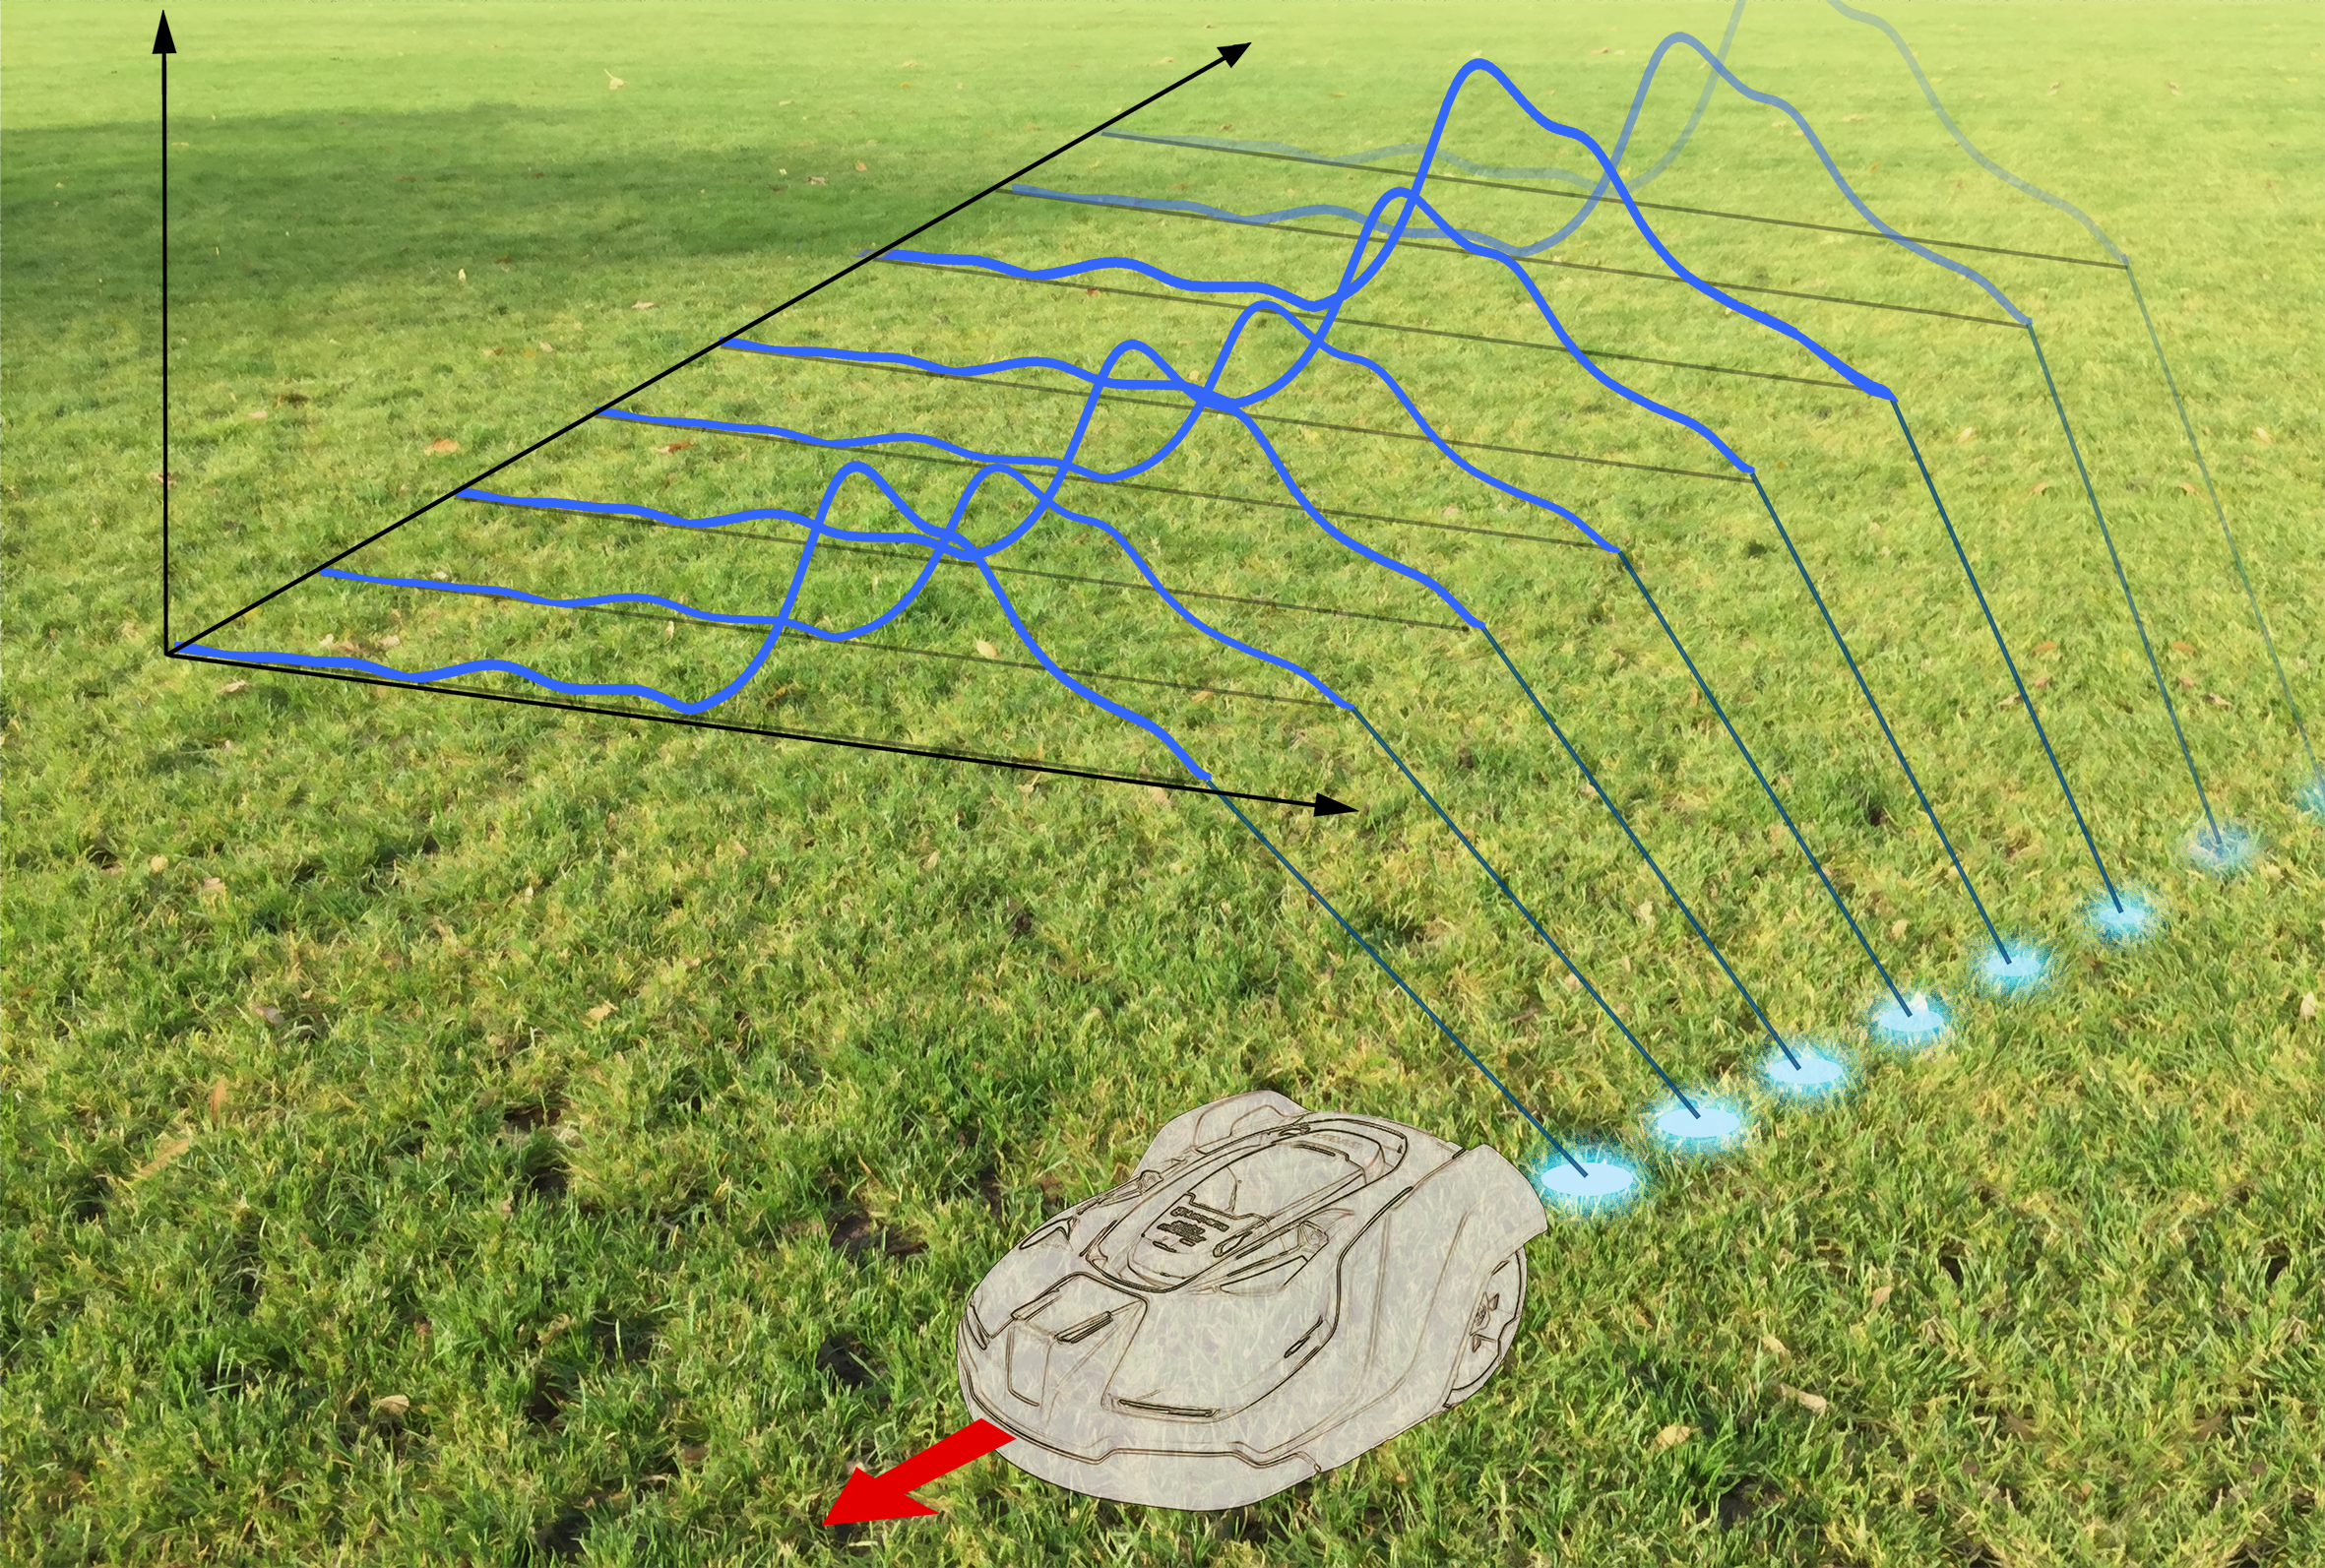
\includegraphics[scale=0.60]{figs_temp/data_collecting.jpg}
	\caption{Two sensors mounted at the front of a robot collect data while the robot is moving forward. Note that the collected data is of IQ-form, whereas the image depicts its absolute values for the sake of clarity.}
	\label{fig:data_collecting}
\end{figure}

\subsection*{Measurement Setup}
The measurement setup is comprised of two sensors, mounted at the front of \emph{a slowly moving robot}. One of the sensors is facing straight down towards the ground, whereas the other one is tilted 22.5 degrees, facing forward. The idea behind this setup is that the two sensors will capture information about the same surface but from different directions. 

Say for example we are presented two surfaces with equivalent reflective properties but where one is rugged and the other is smooth. For the smooth surface the reflections behave more predictably than those for the rugged. If a strong electromagnetic pulse is transmitted from the sensor facing down, one would expect to receive a strong response from the smooth surface. If one instead were to transmit a pulse from the tilted sensor, the opposite would be expected as the reflections upon the smooth surface would primarily bounce away from the sensor, yielding a weak response.

For the rough surface on the other hand, the signal would scatter in a wider array of angles, both when the pulse is transmitted from the flat and the tilted sensor. An idealization of what the received reflection amplitudes could look like from the four scenarios (2 surfaces, and 2 sensors) is presented in figure \ref{fig:reflections}.

\begin{figure}[h]
	\centering
	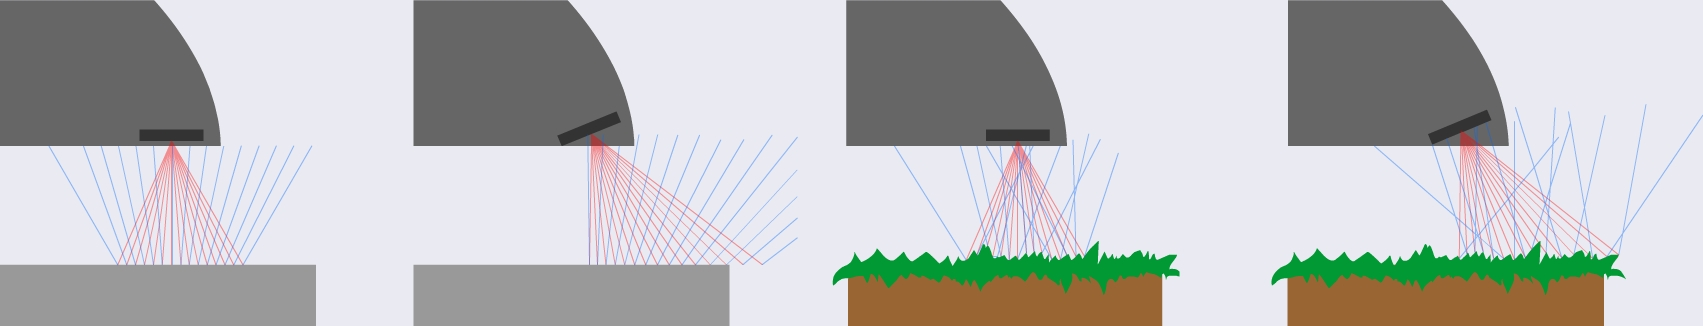
\includegraphics[scale=0.9]{figs_temp/reflections.jpg}
	\caption{Using two sensors mounted with different tilts, we can get information about a surface's roughness. For a smooth surface, the flat and tilted sensors yield a very different response, whereas for a rugged surface the responses are more similar.}
	\label{fig:reflections}
\end{figure}

Possibly mention the $\frac14\lambda$ gap between the sensor and RLM plastic.


\subsection*{Measurement Settings}
Setting the sensor parameters is an iterative process which requires a trial-and-error approach. However, the choices for some parameters can be narrowed down with a little bit of thought. One such parameter is the sampling frequency. When working with means that could potentially cause aliasing, such as the DFT \citep{lindgren_rootzeŽn_sandsten_2013}, it is important to choose a sampling frequency high enough to avoid this.

In order to assure that aliasing is avoided, the maximal frequency component registered by the radar must be surpassed by half the sampling frequency \footnote{This is often referred to as the Nyquist frequency, and is defined as $f_N=f_s/2$.}.
\begin{equation}
\label{eq:nyquist}
	f_{max} < \frac{f_s}2.
\end{equation}
The sampling frequency can be chosen accordingly, assuming the maximal frequency component is known. 

In figure \ref{fig:sensor_placement}, a vehicle is moving forward with constant speed, $v_0$, having a sensor mounted at the front with a 22.5 degree tilt, and a 60 degree beamwidth. As it moves forward, small objects on the ground get closer to the radar sensor with velocity, $v_0$. The maximal velocity component that is orthogonal to the sensor occurs at the far end of the radar's view, and is computed as $v_{\perp, max} = v_0\cdot \cos(37.5^\circ)$.

The movements orthogonal to the radar give rise to doppler frequencies that are registered by the radar. These frequencies are \citep{lien_gillian_karagozler_amihood_schwesig_olson_raja_poupyrev_2016}
\begin{equation}
	f_{d} = \frac{2v_\perp}{\lambda}.
\end{equation}
With $v_0=0.3$ m/s, and $\lambda \approx 0.005$ m, the maximal doppler frequency that can occur is given by 
\begin{equation}
	f_{d,\textrm{max}} = \frac{2\cdot v_{\perp, \textrm{max}}}{\lambda} \approx 95.20.
\end{equation}
Combining this result with equation \eqref{eq:nyquist}, we see that we have to choose a sampling frequency which satisfies
\begin{equation}
	f_s > 2f_{d,\textrm{max}} = 190.4.
\end{equation}
We concluded that $f_s=200$ Hz is a good trade-off between avoiding aliasing, as well as package loss and still maintaining a good time resolution.

\begin{figure}[h]
	\centering
	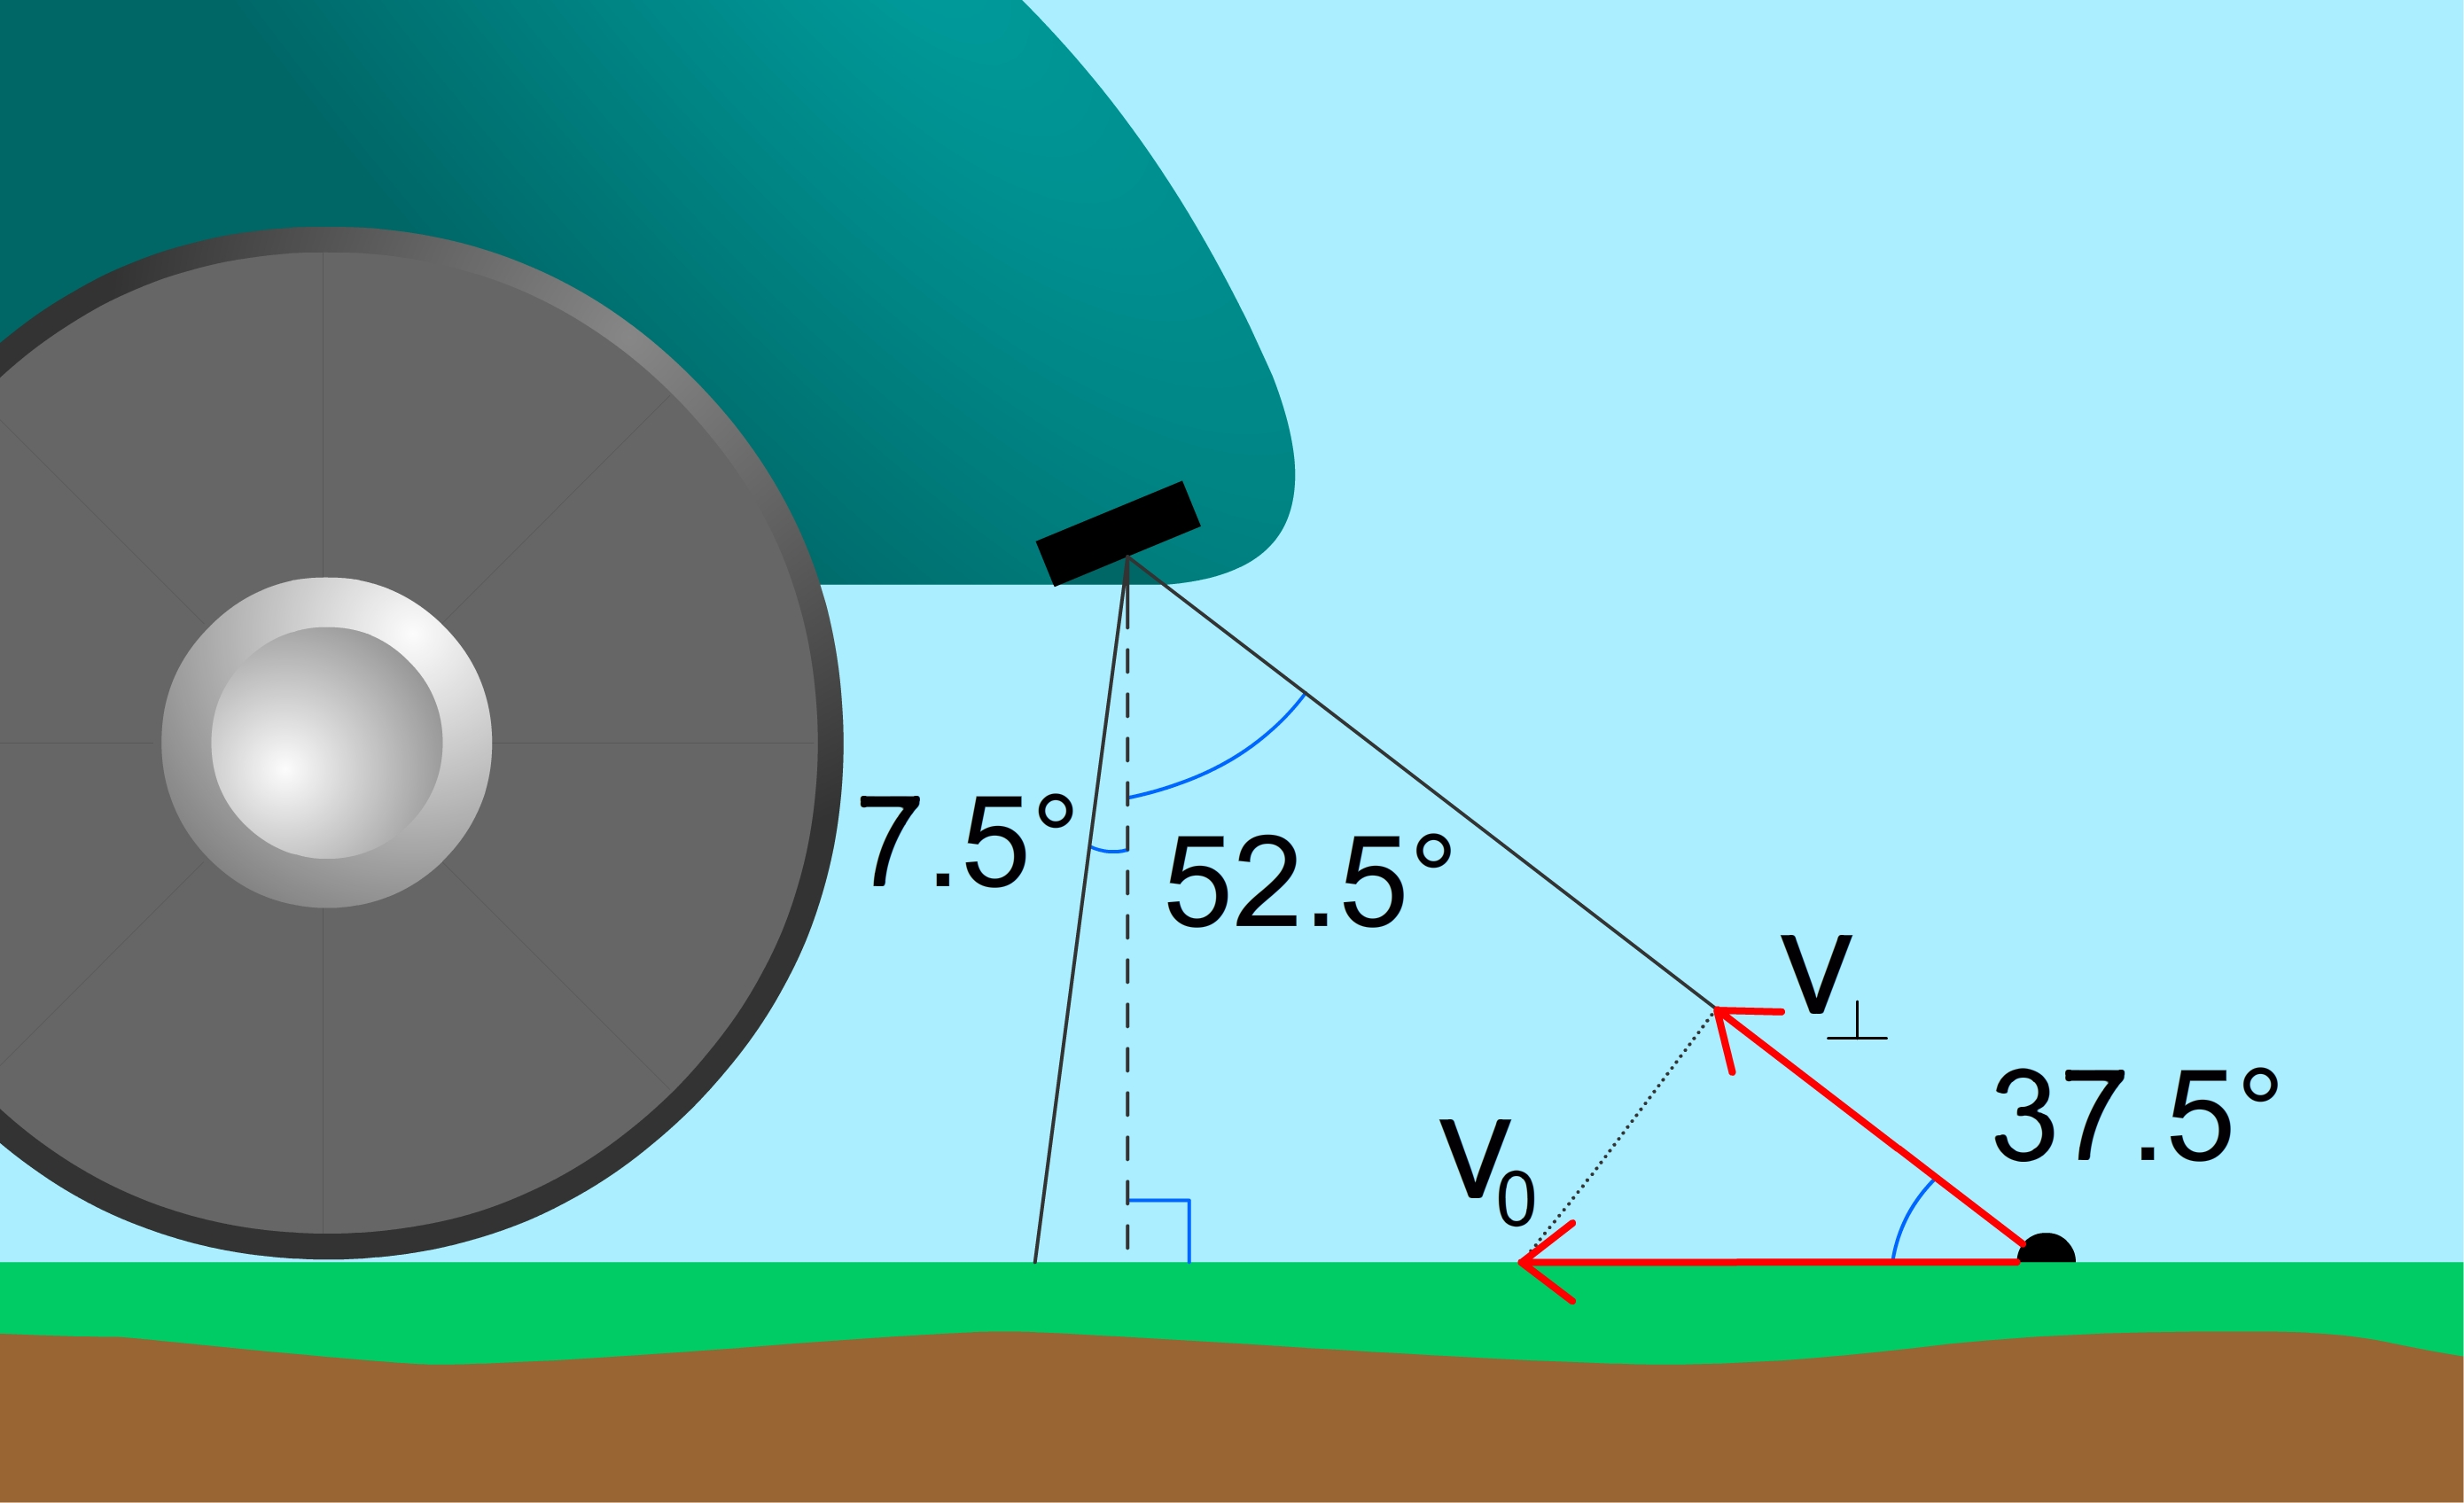
\includegraphics[scale=0.30]{figs_temp/sensor_placement.jpg}
	\caption{}
	\label{fig:sensor_placement}
\end{figure}

\section{Data Preprocessing}
\subsection{Downsampling}

In an information theoretic framework we interpret a random variable by how unpredicable or unstructured an observation of the variable is\citep{anderson_johnnesson_2006}. First introduced by Claude E. Shannon in his monumental 1948 papers, information theory brings about a mean to quantify the information content of some source \citep{shannon_1948}. This concept, which essentially concerns examining the randomness of a variable, is commonly measured through entropy. Directly related to entropy is mutual information which asserts how much information each member of a set have on the other members. \citep{hyvasrinen_karhunen_oja_2004}. Ideally one wants measurements that have a low measure of mutual information, meaning that each datapoint contain information not found elsewhere in the set. 

Observing a typical radar sweep (figure \ref{fig:singel_sweep}) we note that points are very closely related on a small range scale, and nearly identical if we were to examine them on a sample by sample basis. One could argue that the mutual information found in the set is very high and that the entropy in each datapoint is low. Hence, to lower the first and increase the latter, one could downsample by some factor $D$ in range without significant loss of information.
As mentioned in chapter *information theory chapter*, the correlation between neighboring range samples is very high, which means we can downsample without significant loss of information. The downsampling process essentially requires three hyperparameters: A starting range $R_{start}$ and an end range $R_{end}$ where we begin and end our downsampling process respectively, as well as a downsampling factor $D$.

\begin{equation}
	x_D(n, t) = x(R_{start} + nD, t) \quad \text{for}\quad n=0...\frac{R_{end}-R_{start}}{D}
\end{equation}

\subsection{Sweep Normalization}
The gain of Acconeer radars can vary significantly from one sensor to another. Despite facing towards the very same surface, two sensors may exhibit a similar sweep structure,  yet with very different amplitudes. This could potentially have serious consequences if not handled properly. Assuming a model's training data has been collected with one sensor, it would be impossible to successfully perform classifications with this model using a sensor which has a very different gain. The recordings would simply have too little resemblence, even though they merely differ by a constant gain factor.

A way to combat this problem is to perform some kind of sweep normalization before proceeding with any other processing. There are numerous ways of doing this. A rather simplistic strategy could be to simply normalize each sweep with its maximum value. While this may intuitively seem like a good idea, it may eliminate possible correlations between consecutive samples, as this normalization method only takes one sweep in regard. 

A more robust solution is to have the normalization method depend on several consecutive sweeps. By computing the average energy in all range bins and a number of sweeps, we can normalize all these selected sweeps with this value, and thus maintain their relative structure.

\section{Data exploration}


Good source on PCA
\cite{hyvasrinen_karhunen_oja_2004}
PCA 125-143

Information theory
105-122

Observing a typical radar sweep (figure \ref{fig:singel_sweep}) we note that points are very closely related on a small range scale, and nearly identical if we were to examine them on a sample by sample basis. One could argue that the mutual information found in the set is very high and that the entropy in each datapoint is low. Hence, to lower the first and increase the latter, one could downsample by some factor $D$ in range without significant loss of information.


PCA 125-143: Through the point and feature selection methods described in previous sections we obtain high dimensional feature vectors. Getting an intuitive feel for such data extracted in these processes is difficult as direct plotting is limited to three dimensions. 

Principal Component Analysis (PCA) is  a classical technique in statistical data analysis which takes a large set of multivariate variables and finds a smaller set of variables with less redundancy. Critically, PCA finds a rotated orthogonal coordinate system such that the elements of the set become uncorrelated. Projecting elements on the principal axes corresponding to the directions of maximal variance a good approximation of the original data in lower dimension is obtained \citep{hyvasrinen_karhunen_oja_2004}.

%\iffalse
\begin{figure}[h]
	\centering
	\includegraphics[scale=0.60]{figs_temp/pca_analysis.png}
	\caption{A single radar sweep which has been measured from 7 to 23 cm. The large amplitude at around 13.4 cm. suggests there is some object present at that distance from the sensor.}
	\label{fig:pca}
\end{figure}
%\fi
